\section{Refinar o ciclo de vida do produto e clientes do projeto}\label{sec:refinar_ciclo_de_vida}
Após a definição do problema, uma das primeiras etapas que devem ser realizadas é a definição do ciclo de vida do produto. Os modelos de ciclo de vida representam graficamente a trajetória de um produto, desde os primeiros esforços para sua criação até o encerramento do suporte oferecido pela empresa. Esse ciclo não termina necessariamente com o fim da fabricação ou das vendas, pois produtos podem continuar em uso por muitos anos. Para a empresa, o ciclo se encerra quando termina seu compromisso de pós-venda, incluindo a descontinuação da fabricação, a venda dos estoques e o fornecimento de peças de reposição. Dessa forma, é necessário planejar a disponibilidade de componentes e ferramentas durante o período de transição.



Ao longo das etapas do ciclo de vida do produto, serão identificados e descritos os diferentes tipos de clientes envolvidos no processo. Para cada etapa, serão considerados os clientes internos, que participam diretamente das atividades dentro da organização; os clientes intermediários, que atuam na distribuição ou transformação do produto até seu destino final; e os clientes externos, que representam os usuários ou consumidores finais do produto. Essa abordagem permitirá compreender as necessidades e expectativas de cada grupo ao longo do ciclo de vida

\subsection{Ciclo de Vida}\label{subsec:refinar_ciclo_de_vida}
De modo geral, o ciclo de vida de um produto é composto pelas etapas de desenvolvimento, lançamento, crescimento, maturidade e declínio, que representam sua evolução desde a concepção até sua retirada do mercado, conforme na figura abaixo.


\begin{figure}[H]
    \centering
    \caption{Ciclo de vida padrão de um produto}
    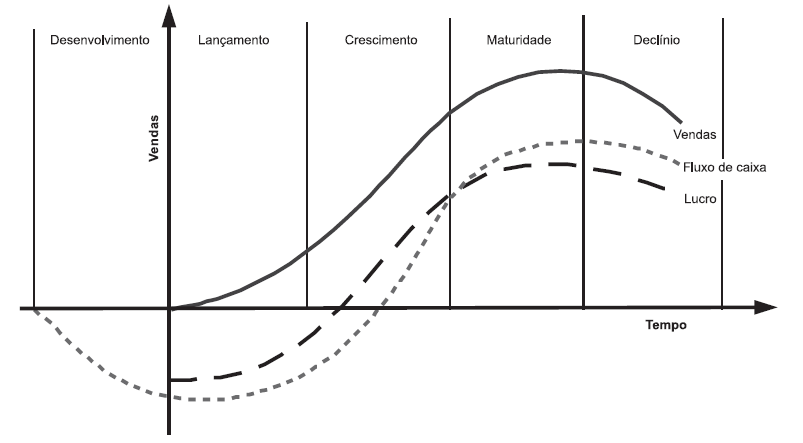
\includegraphics[width=0.8\textwidth]{imagens/refinar ciclo de vida/fig01-ciclo-de-vida-padrao.png}
    \label{fig:ciclo-de-vida-teorico}
    \source{\cite{rozenfeld2006gestao}}
\end{figure}




Entretanto, no contexto deste projeto, o ciclo de vida será consideravelmente mais curto, uma vez que o objetivo é desenvolver apenas um protótipo e, possivelmente, realizar testes com pequenas quantidades do produto. Dessa forma, não haverá uma produção em larga escala ou uma comercialização efetiva.

Além disso, como não está prevista a venda dos produtos desenvolvidos, não haverá geração de receitas ao longo do ciclo de vida. Assim, o fluxo de caixa do projeto será predominantemente composto por saídas de recursos, relacionadas ao desenvolvimento, produção do protótipo e realização dos testes, sem a correspondente entrada de receitas proveniente de vendas. Portanto, as etapas tradicionais de crescimento e maturidade serão bastante reduzidas ou até mesmo inexistentes, fazendo com que o ciclo se concentre principalmente no desenvolvimento, lançamento experimental e posterior encerramento do projeto.

\begin{figure}[H]
    \centering
    \caption{Ciclo de vida esperado do produto}
    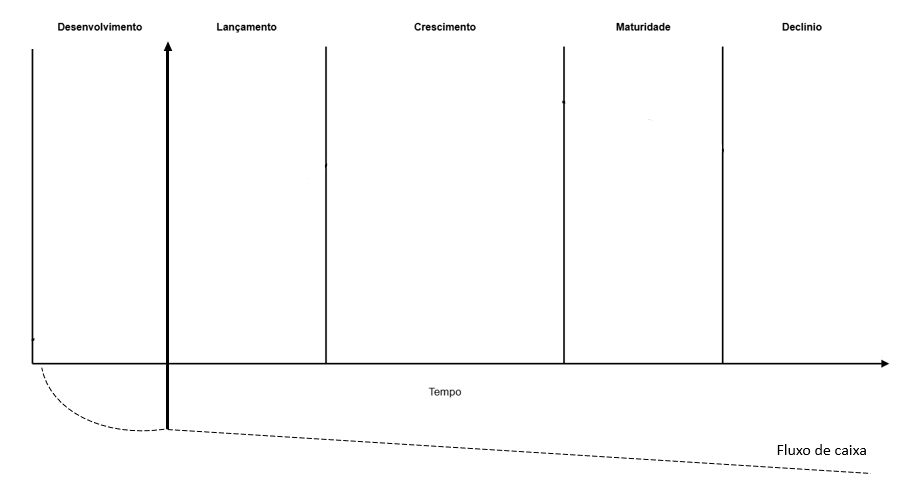
\includegraphics[width=0.8\textwidth]{imagens/refinar ciclo de vida/fig02-ciclo-de-vida-real.png}
    \label{fig:ciclo-de-vida-nosso-produto}
    \source{Autoria Própria}
\end{figure}


\subsubsection{Ciclo de Vida segundo as atividades}
\label{subsubsec:ciclo_vida_padrao}

\paragraph{Planejamento estratégico:}
\label{par:planejamento_estrategico}

Nesta etapa, é realizada a identificação do problema e das necessidades existentes no mercado. No contexto do projeto, observa-se que o processo tradicional de pagamento no varejo de roupas pode envolver filas, deslocamentos até os caixas e diferentes etapas que aumentam o tempo necessário para concluir uma compra. A partir dessa necessidade, identifica-se a oportunidade de desenvolver uma solução que torne o processo de pagamento mais rápido e conveniente para o consumidor, ao mesmo tempo em que possa contribuir para a eficiência operacional das lojas. A análise considera o contexto do varejo de roupas, tendo a Riachuelo como uma referência para compreensão do problema, sem limitar a solução exclusivamente à empresa.

\paragraph{Planejamento do produto:}
\label{par:planejamento_produto}

Após a identificação do problema, são definidos os principais requisitos e características que o produto deverá apresentar para atender às necessidades identificadas. Nesse projeto, a solução será composta por dois elementos principais: uma tag (bolacha) equipada com um identificador RFID/QR Code e um mecanismo de eletroímã, e um aplicativo responsável pela leitura da tag e pelo processo de pagamento. O planejamento busca estabelecer como esses componentes deverão funcionar de forma integrada, considerando aspectos como facilidade de utilização pelo consumidor, segurança, viabilidade técnica e adequação ao ambiente do varejo.

\paragraph{Projeto:}
\label{par:projeto}

Na etapa de projeto, os requisitos definidos anteriormente são transformados em uma solução técnica detalhada. São desenvolvidos o conceito e a estrutura da tag, incluindo o sistema RFID/QR Code e o mecanismo que permitirá seu desprendimento da roupa após a confirmação do pagamento. Paralelamente, é projetado o aplicativo responsável pela identificação da peça, interação com o usuário e comunicação necessária para confirmar a transação. Também são definidas as interfaces entre os componentes físicos e digitais, buscando garantir que o funcionamento do sistema seja integrado.

\paragraph{Planejamento do processo:}
\label{par:planejamento_processo}

Com o produto definido, é necessário determinar como ele será desenvolvido e produzido. Nesta etapa, são estabelecidos os materiais, componentes, ferramentas e procedimentos necessários para a montagem da tag e o desenvolvimento do aplicativo. Como o projeto possui caráter acadêmico e será desenvolvido em pequena escala, o planejamento do processo será direcionado principalmente à produção dos protótipos, e não à fabricação em massa. Também devem ser consideradas a sequência de montagem, a integração dos componentes e os procedimentos necessários para verificar o funcionamento da solução durante sua construção.

\paragraph{Produção:}
\label{par:producao}

A etapa de produção corresponde à fabricação dos componentes físicos e à implementação dos elementos necessários para o funcionamento do sistema. No projeto, essa etapa será limitada à produção de uma pequena quantidade de unidades, suficiente para a realização dos testes e demonstração da solução. A montagem envolverá a integração do identificador RFID/QR Code, do eletroímã e dos demais componentes necessários ao funcionamento da tag. Paralelamente, será realizada a implementação do aplicativo e sua integração com o sistema desenvolvido.

\paragraph{Prototipagem:}
\label{par:prototipagem}

A prototipagem consiste na materialização da solução planejada em um modelo funcional, permitindo avaliar, de forma prática, se os conceitos definidos nas etapas anteriores são tecnicamente viáveis. Neste projeto, serão desenvolvidos protótipos da tag RFID/QR Code e do aplicativo, buscando reproduzir, em escala reduzida, o funcionamento esperado da solução final. A prototipagem também permitirá identificar dificuldades de montagem, integração entre hardware e software e possíveis melhorias no produto antes da realização dos testes.

\paragraph{Testes:}
\label{par:testes}

Por fim, serão realizados testes para verificar o funcionamento e o atendimento aos requisitos estabelecidos para o produto. O sistema será avaliado considerando o processo completo: identificação da peça por meio do RFID/QR Code, utilização do aplicativo, confirmação do pagamento e acionamento do eletroímã para liberação da tag. Como não haverá produção em massa, os testes serão realizados em pequena escala, utilizando os protótipos desenvolvidos. Os resultados obtidos poderão indicar falhas, limitações ou oportunidades de melhoria, permitindo avaliar a viabilidade da solução e propor ajustes no produto.




\subsection{Definição dos clientes do projeto - Cliente, Usuário, Mercado e Segmento}\label{subsec:definicao_dos_clientes}

\subsubsection{Cliente}
\label{subsubsec:cliente}

O cliente do projeto é a entidade que realiza a transação comercial relacionada à aquisição do produto ou serviço. No contexto da solução desenvolvida, os principais clientes são as empresas do setor varejista de roupas que adotarem o sistema como parte de seu processo de vendas. Essas empresas serão responsáveis pela aquisição e implementação da solução, composta pela tag RFID/QR Code e pelo aplicativo, visando aprimorar o processo de pagamento e proporcionar maior eficiência às operações de suas lojas.

Considerando a segmentação demográfica, os clientes são caracterizados principalmente como pessoas jurídicas, com diferentes portes e estruturas organizacionais. Já a segmentação geográfica inicialmente considerada para o projeto corresponde ao mercado brasileiro, de modo que a solução seja desenvolvida considerando as características e necessidades do varejo de roupas no Brasil, mais especificamente São Paulo. A Riachuelo é utilizada como referência para o desenvolvimento do projeto, porém a solução não será exclusiva para essa empresa, podendo ser aplicada a outros varejistas que apresentem necessidades semelhantes.

\subsubsection{Usuário}
\label{subsubsec:usuario}

O usuário é a entidade que utiliza diretamente os produtos ou serviços oferecidos. No projeto, os principais usuários são os consumidores finais das lojas de roupas, que utilizarão o aplicativo para realizar o processo de pagamento. O consumidor deverá utilizar o aplicativo para identificar a peça de roupa por meio do RFID/QR Code e realizar ou confirmar o pagamento. Após a confirmação da transação, o sistema acionará o eletroímã presente na tag, permitindo que a peça seja liberada.

Os usuários são, portanto, predominantemente pessoas físicas. Em relação à segmentação demográfica, a solução poderá atender consumidores de diferentes faixas etárias, gêneros e níveis de renda, desde que possuam acesso a um dispositivo compatível com o aplicativo. Quanto à segmentação geográfica, inicialmente considera-se o território brasileiro, com foco em consumidores que realizam compras em estabelecimentos do varejo de roupas que adotem a solução.

Além dos consumidores, funcionários das lojas também poderão ser considerados usuários indiretos do sistema, uma vez que estarão envolvidos na disponibilização das tags, no acompanhamento das operações e no suporte aos consumidores durante a utilização da solução.

\subsubsection{Mercado}
\label{subsubsec:mercado}

O mercado corresponde ao conjunto de compradores reais e potenciais dos produtos ou serviços oferecidos. Para o projeto, o mercado é constituído principalmente pelas empresas que atuam no varejo de roupas e que possuem interesse em soluções capazes de tornar o processo de pagamento mais rápido e eficiente. Nesse contexto, enquadram-se tanto grandes redes varejistas quanto empresas de menor porte que possam incorporar tecnologias de automação ao processo de vendas.

Do ponto de vista demográfico, por se tratar de um mercado predominantemente B2B (\textit{business-to-business}), sua caracterização está mais relacionada às características das empresas, como porte, quantidade de lojas, volume de vendas e nível de adoção tecnológica, do que às características individuais dos compradores.

A solução apresenta potencial de aplicação em diferentes estabelecimentos do varejo de roupas, uma vez que o problema relacionado à agilidade e eficiência do processo de pagamento pode ocorrer independentemente do porte específico da empresa.

\subsubsection{Segmento de mercado}
\label{subsubsec:segmento_mercado}

O segmento de mercado representa uma subdivisão do mercado em grupos que apresentam características e necessidades semelhantes. Para este projeto, o principal segmento definido é o de empresas do varejo de roupas que buscam soluções tecnológicas para automatizar e agilizar o processo de pagamento em suas lojas físicas.

Considerando a segmentação demográfica, o projeto pode priorizar empresas de médio e grande porte, especialmente redes varejistas que possuam elevado fluxo de consumidores e um número significativo de peças comercializadas. Essas características tornam os ganhos relacionados à redução do tempo de pagamento e à automação do processo potencialmente mais relevantes.


